
\documentclass[oneside]{diretrizes}            % Imprimir apenas frente
%\documentclass[doubleside]{diretrizes}        % Imprimir frente e verso

% Importações de pacotes
\usepackage[alf, abnt-emphasize=bf, recuo=0cm, abnt-etal-cite=2, abnt-etal-list=0]{abntex2cite}  % Citações padrão ABNT
\usepackage[utf8]{inputenc}                         % Acentuação direta
\usepackage[T1]{fontenc}                            % Codificação da fonte em 8 bits
\usepackage{graphicx}                               % Inserir figuras
\usepackage{amsfonts, amssymb, amsmath}             % Fonte e símbolos matemáticos
\usepackage{booktabs}                               % Comandos para tabelas
\usepackage{verbatim}                               % Texto é interpretado como escrito no documento
\usepackage{multirow, array}                        % Múltiplas linhas e colunas em tabelas
\usepackage{indentfirst}                            % Endenta o primeiro parágrafo de cada seção.
\usepackage{microtype}                              % Para melhorias de justificação?
\usepackage[algoruled, portuguese]{algorithm2e}     % Escrever algoritmos
\usepackage{float}                                  % Utilizado para criação de floats
\usepackage{times}                                  % Usa a fonte Times

% Inclui o preâmbulo do documento
%
% Documento: Preâmbulo
%

\instituicao{Instituto Federal de Educação, Ciência e Tecnologia \\do Rio Grande do Sul}
\abreviatura{IFRS}
\departamento{Campus Restinga}
\local{Porto Alegre}
\programa{Análise e Desenvolvimento de Sistemas}
\nomeautor{Felipe dos Santos Viegas}
\titulotb{Pybot}
%\subtitulo{Subtítulo do trabalho}
\data{2017}
\grau{Tecnólogo}
\dataapresentacao{DD/MM/20AA}

%Dados Orientador
\orientador{Roben Castagna Lunardi}
%\coorientador{Anderson Black}
\instOrientador{IFRS}
\departamentoorientador{Campus Restinga}
\titulacaoorientador{Prof. Me.}

%Dados Coorientador
%\coorientador{Artur Dent}
%\instCoorientador{IFRS}
%\departamentocoorientador{Campus Restinga}
%\titulacaocoorientador{Prof. Dr.}

%Dados Examinador 1
\nmexamum{Mestre dos Magos}
\instexamum{IFRS}
\departamentoexamum{Campus Restinga}
\titulacaoexamum{Prof.}

%Dados Examinador 2
\nomeexamdois{Mestre Splinter}
\instexamdois{IFRS}
\departamentoexamdois{Campus Restinga}
\titulacaoexamdois{Prof. Me.}


% Define as cores dos links e informações do PDF
\makeatletter
\hypersetup{
    portuguese,
    colorlinks,
    linkcolor=black,
    citecolor=black,
    filecolor=black,
    urlcolor=black,
    breaklinks=true,
    pdftitle={\@title},
    pdfauthor={\@author},
    pdfsubject={\imprimirpreambulo},
    pdfkeywords={abnt, latex, abntex, abntex2}
}
\makeatother

% Redefinição de labels
\renewcommand{\algorithmautorefname}{Algoritmo}
\def\equationautorefname~#1\null{Equa\c c\~ao~(#1)\null}

% Cria o índice remissivo
\makeindex

% Início do documento
\begin{document}

    % Retira espaço extra obsoleto entre as frases.
    \frenchspacing

    % Elementos pré textuais
    \pretextual
    %
% Documento: Capa
%

\makeatletter
\begin{capa}
	\thispagestyle{empty}%limpa estilo da pagina
	\setlength{\baselineskip}{0.72\baselineskip}
    \begin{center} %Alinhamento centralizado
	

    \textbf{\expandafter\uppercase\expandafter{\imprimirinstituicao}}\\
    \textbf{\expandafter\uppercase\expandafter{\imprimirdepartamento}}\\
    \textbf{\expandafter\uppercase\expandafter{\imprimirprograma}}\\
	\vspace*{5cm}%Espaçamento entre linhas
	\large\textbf{\expandafter\uppercase\expandafter{\imprimirtitulotb}}\\
	\vspace*{6cm}%Espaçamento entre linhas	
	\small\textbf{\expandafter\uppercase\expandafter{\imprimirnomeautor}}\\
	\vspace*{9.5cm}%%Espaçamento entre linhas
	\small\textbf{\expandafter\uppercase\expandafter{\imprimirlocal}}\\
	\small\textbf{\expandafter\uppercase\expandafter{\imprimirdata}}\\
		
		
		
	\end{center} %Alinhamento centralizado
\end{capa}
\makeatother

	

              % Capa
    %
% Documento: FOLHA DE ROSTO
%

\makeatletter
\begin{folhaderosto}
	\thispagestyle{empty}%limpa estilo da pagina
	
    \begin{center}
    
		\small\textbf{\expandafter\uppercase\expandafter{\imprimirnomeautor}}\\
		\vspace*{8.2 cm}%Espaço entre linhas
		\normalsize\textbf{\expandafter\uppercase\expandafter{\imprimirtitulotb}}\\
		
    \end{center}
	
	\vspace*{0.35 cm}%Espaçamento entre linhas
		    \large%tamanho da fonte 
    		\hfill%Estica horizontamente  com espaços
	    	\begin{minipage}{8 cm}%Minipagina
	    		\begin{small} %Muda tamanho da fonte
	    		\setlength{\baselineskip}{0.7\baselineskip}
				
		    	{Trabalho de Conclusão de Curso apresentada como requisito parcial para obtenção do grau de
		    	{\imprimirgrau } em {\imprimirprograma } da {\imprimirinstituicao}{ - }{\imprimirabreviatura},
		    	{\imprimirdepartamento}.}\\{
		    	}\\Orientador: {\imprimirtitulacaoorientador }{ }{\imprimirorientador}\\{
		    	}\\Co-orientador: {\imprimirtitulacaocoorientador }{ }{\imprimircoorientador}
				
				
				\end{small} %Muda tamanho da fonte
		    \end{minipage}%%Minipagina
		    	
		    \vspace*{10 cm}%Espaçamento entre linhas
		    
		    \begin{center} %Alinhamento centralizado
		    	\normalsize %Muda tamanho da fonte
	    		\imprimirlocal\\
	    		\imprimirdata
	    	\end{center}%Alinhamento centralizado

\end{folhaderosto}
\makeatother
        % Folha de rosto
    %
% Documento: FOLHA APROVAÇÃO
%

\makeatletter
\begin{folhadeaprovacao}

\thispagestyle{empty}%limpa estilo da pagina
	
	\begin{center}
    
		\small\textbf{\expandafter\uppercase\expandafter{\imprimirnomeautor}}\\
		\vspace*{3.0 cm}%Espaço entre linhas
		\normalsize\textbf{\expandafter\uppercase\expandafter{\imprimirtitulotb}}
		
    \end{center}
	
	\vspace*{0.35 cm}%Espaçamento entre linhas
		    \large%tamanho da fonte 
    		\hfill%Estica horizontamente  com espaços
	    	\begin{minipage}{8 cm}%Minipagina
	    		\begin{small} %Muda tamanho da fonte
	    		\setlength{\baselineskip}{0.7\baselineskip}
				
		    	{Trabalho de Conclusão de Curso apresentado como requisito parcial para obtenção do grau de
		    	{\imprimirgrau } em {\imprimirprograma } do {\imprimirinstituicao}{ - }{\imprimirabreviatura},
		    	{\imprimirdepartamento}.}\\{
		    	}\\				
				
				\end{small} %Muda tamanho da fonte
		    \end{minipage}%%Minipagina
		    	
		    \vspace*{0.6 cm}%Espaçamento entre linhas
		    
		    \large%%tamanho da fonte 
    		\hfill%%Estica horizontamente  com espaços
	    	 
		    
		    \normalsize %Muda tamanho da fonte
		    \vspace*{1.5 cm}%Espaçamento entre linhas
		    
		    \begin{minipage}{9 cm }%%Minipagina
		    {Data de Aprovação: {\imprimirdataapresentacao}}\\
		    \end{minipage}%Minipagina
			
			\begin{center}%Alinhamento centralizado
		    	\vspace*{1.21 cm}%Espaçamento entre linhas
				\textbf{Banca Examinadora}\\ %Negrito
						
				\vspace*{1 cm}%Espaçamento entre linhas
				\rule{9 cm}{.1 mm}\\
				{\imprimirtitulacaoorientador}{ }{\imprimirorientador} - {\imprimirinstOrientador} - {\imprimirdepartamentoorientador}\\
				Orientador\\
				
				\vspace*{1 cm}%Espaçamento entre linhas
				\rule{9 cm}{.1 mm}\\
				\imprimirtitulacaoexamum{ }\imprimirnmexamum - \imprimirinstexamum - \imprimirdepartamentoexamum\\
				Membro da Banca
				
				\vspace*{1 cm}%Espaçamento entre linhas
				\rule{9 cm}{.1 mm}\\				
								
				\imprimirtitulacaoexamdois{ }\imprimirnomeexamdois - \imprimirinstexamdois - \imprimirdepartamentoexamdois\\
				Membro da Banca
				\vspace*{1.3 cm}%Espaçamento entre linhas
		    \end{center}%Alinhamento centralizado


\end{folhadeaprovacao}
\makeatother
    % Folha de aprovação
    %
% Documento: Folha Catalográfica
%

\thispagestyle{empty}
\vspace*{\fill}

 \begin{flushleft}
\small \setlength{\baselineskip}{0.8\baselineskip}INSTITUTO FEDERAL DE EDUCAÇÃO, CIÊNCIA E TECNOLOGIA DO RIO GRANDE DO SUL\\
Reitor: Prof. Osvaldo Casares Pinto\\
Pró-Reitora de Ensino: Profa. Clarice Monteiro Escott\\
Diretor do Campus Restinga: Prof. Gleison Samuel do Nascimento\\
Coordenador do Curso de Ciência da Computação: Prof. Rafael Pereira Esteves\\
Bibliotecária-Chefe do Campus Restinga: Paula Porto Pedone\\
\end{flushleft}



    %
% Documento: Dedicatória
%

\thispagestyle{empty}
\begin{dedicatoria}

Dedico esse trabalho a todos aqueles que me ajudaram do fim ao começo!

\end{dedicatoria}
       % Dedicatória
%    %
% Documento: Agradecimento
%

\begin{agradecimento}

Neste trecho você faz agradecimentos dirigidos aqueles que contribuíram de maneira relevante a elaboração do trabalho.
Elemento opcional segundo a norma da ABNT NBR 14724 de 2011.

\end{agradecimento}

    % Agradecimentos
    %
% Documento: Epígrafe
%
\thispagestyle{empty}
\begin{epigrafe}


O fator decisivo para vencer o maior obstáculo é, invariavelmente, ultrapassar o obstáculo anterior.{\\}{\\}

\begin{autorepigrafe}
Henry Ford
\end{autorepigrafe}

\end{epigrafe}


          % Epígrafe
    %
% Documento: Resumo (Português)
%

\begin{RESUMO}
\thispagestyle{empty}
	\begin{SingleSpace}


		Em muitas empresas temos uma certa carência quando o assunto é automação de testes ou processos web em navegadores. A necessidade de testes de regressão, testes de funcionalidades e ou
        automação de processos cresce junto com o sistema, porem a pratica dessas atividades só tem força quando aparece aguma necessidade ou problema.

        Esse novo framework pretende trazer aos usuarios uma ferramenta de facil uso e com recursos uteis para o desenvolvimento dessas tarefas, contando com a facilidade e versatilidade da
        linguagem python e a integração com navegadores com framework selenium.

        O conjuntos de ferarmentas que o framework dispõe são: gerenciamento automatico dos controladores de navegadores(drivers), modulo de relatorios e logs para controle de atividades executadas,
        padronização de criação de elementos de tela utilizando o padrão PageObject.

		\vspace*{0.5cm}\hspace{-1.3 cm}\textbf{Palavras-chave}: Automação, Selenium, Testes.

	\end{SingleSpace}
\end{RESUMO}


          % Resumo na língua vernácula
    %
% Documento: Resumo (Inglês)
%

\begin{ABSTRACT}
	\begin{SingleSpace}


        Currently, many companies lack a solution for  test automation or web process management integrated to the browsers.
        The need for regression testing, functionality testing, and / or process automation grows along with the system,
        but the practice of these activities is only emerge when a need or problem appears.

        In order to solve this problem, we propose a framework aims to present to  users an easy-to-use tool with useful resources for the development of these
        tasks, with the simplicity and versatility of the \textit{Python} language and the integration with browsers with \textit{selenium framework}.

        The sets of tools that the proposed framework presents are: automatic management of the drivers of navigators (\textit{drivers}); module containing reports
        and logs to control activities performed; standardization of screen elements development using the standard \textit{PageObject} and identification of layout change.

		\vspace*{0.5cm}\hspace{-1.3 cm}\textbf{Palavras-chave}: Automation, Selenium, Tests.


	\end{SingleSpace}

\end{ABSTRACT}
          % Resumo em língua estrangeira
    %
% Documento: Lista de figuras
%

\pdfbookmark[0]{\listfigurename}{lof}
\listoffigures*
\cleardoublepage

      % Lista de figuras
    %
% Documento: Lista de tabelas
%

\pdfbookmark[0]{\listtablename}{lot}
\listoftables*
\cleardoublepage
      % Lista de tabelas
    %
% Documento: Lista de quadros
%

\pdfbookmark[0]{\listofquadrosname}{loq}
\listofquadros*
\cleardoublepage
      % Lista de quadros
    %
% Documento: Lista de abreviaturas e siglas
%

\begin{siglas}
	\setlength{\baselineskip}{0.7\baselineskip}
	
    \item[ABNT] Associação Brasileira de Normas Técnicas
    \item[TCC] Trabalho de Conclusão do Curso
    \item[NBR] Norma Brasileira
\end{siglas}
       % Lista de abreviaturas e siglas
    %%
% Documento: Lista de símbolos
%

\begin{simbolos}
    \item[$ \Gamma $] Letra grega Gama
    \item[$ \lambda $] Comprimento de ondada
    \item[$ \in $] Pertence
\end{simbolos}
     % Lista de símbolos
    \sumario

    % Elementos textuais
    \textual
    %
% Documento: Introdução
%

\chapter{INTRODUÇÃO}\label{chap:introducao}

O ciclo de vida de software tem diveras etapas, de um modo geral elas são: Análise de requisitos, Concepção do Projeto, Desenvolvimento, Implantação e por fim Manutenção.
Nas etapas de Desenvolvimento e a Manutenção é onde a criação ou a codificação do software em questão mais acontece, e na concepção de um projeto a necessidade da criação
de um processo de testes que cresça junto do sistema não tem a sua devida importação.


Este Trabalho de Conclusão de Curso tem como objetivo criar um framework para auxiliar nas tarefas de criação de testes e ou automatização de processos de sistemas executados em navegadores.
Levando o nome de PyBot, união das palavras Python, liguagem utilizada para criação do projeto, e Bot, que em inglês quer dizer robô, essa ferramenta propõe prover para os usuarios uma serie
de ferramentas para auxiliar a criação e implantação desses processos, contando uma estrutura de criação dos scripts de teste no padrão PageObject e PageElement, geração de registros de logs
para controle de tarefas e passos executados, verificação de alteração de interfaces e layout dos sites e o gerenciamento automatico de drivers de navegadores com a ferramenta Driloader.            % Introdução
    %
% Documento: Disposições
%

\chapter{DISPOSIÇÕES GERAIS}

O trabalho deve ser apresentado aos orientadores de TCC. A quantidade de exemplares e as regras de apresentação desses trabalhos devem seguir as normas estabelecidas pelas normas da Universidade.

O documento deve respeitar as normatizações estabelecidas pela Associação Brasileira de Normas Técnicas seguindo o NBR 14724 de 2011.

\section{SEÇÕES E SUBSEÇÕES}

As seções devem utilizar algarismos arábicos de numeração. Limitar a numeração pro-gressiva até a seção quinaria. O título (primarias, secundarias, terciarias, quaternárias e quinari-as) deve ser colocado após o indicativo de seção, alinhado à margem esquerda, separado por um espaço. O texto deve iniciar em outra linha. 

O indicativo das seções primarias deve ser grafado em números inteiros a partir de 1. O indicativo de uma seção secundária é constituído pelo número da seção primaria a que pertence, seguido do número que lhe for atribuído na sequência do assunto e separado por ponto. Repete-se o mesmo processo em relação ás demais seções.

\section{ESPAÇAMENTO}

O texto deve ser digitado em espaço 1,5 – exceto as referências que devem ter espaço 1 – e ocupar apenas o anverso da página. Recomenda-se a utilização da fonte Times New Roman\index{NewR}\footnote{Família tipográfica}, tamanho 12 para o texto e, tamanho 10 para a citação direta de mais de três linhas. Tipos itálicos são usados para nomes científicos e expressões latinas. As citações longas, as notas, as referências e os resumos em vernáculo e em língua estrangeira devem ser digitados em espaço simples. Os títulos das seções devem ser separados do texto que os precede ou que os sucede por uma entrelinha dupla (um espaço duplo ou dois espaços simples).

\section{ALINHAMENTO}

Para efeito de alinhamento, no texto, deve ser utilizado o justificado. A impressão deve ser feita exclusivamente em papel branco formato A4 (21,0 x 29,7cm), de boa opacidade e de qualidade que permita a impressão e leitura.

\section{MARGENS}

As margens devem ser: para o anverso, esquerda e superior de 3 cm e direita e inferior de 2 cm; para o verso, direita e superior de 3 cm e esquerda e inferior de 2 cm.

\section{NUMERAÇÃO}

Todas as folhas a partir da folha de rosto devem ser contadas,porém não numeradas. A numeração deve ser indicada a partir da Introdução, que poderá ser, por exemplo 5, se foram utilizadas quatro folhas anteriormente. Quando forem utilizadas folhas em branco para abrir os capítulos, estas não devem ser contadas para efeito de paginação.

\section{ABREVIATURAS}

As abreviaturas e siglas quando aparecem pela primeira vez no texto, devem ter os no-mes colocados por extenso, acrescentando-se a abreviatura ou a sigla entre parênteses.


           % Disposições
    %
% Documento: Estrutura
%

\chapter{ESTRUTURA}

A estrutura de acordo com a NBR-14724, compreende três elementos: pré-textuais, tex-tuais e pós-textuais.

\begin{figure}[H]
	\vspace*{0,2cm}
    \centering
    \caption{Ilustração da estrutura}
    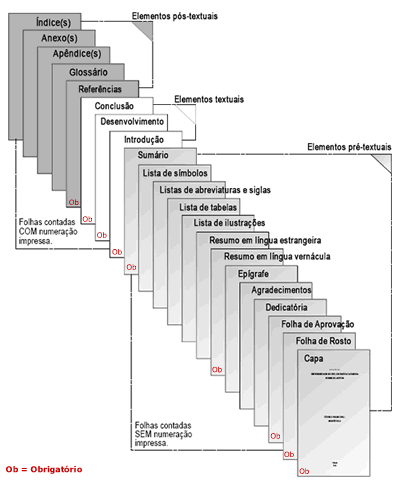
\includegraphics[width=0.6\textwidth]{./04-figuras/abnt}
    \label{fig:ilustfig2}
\end{figure}
\vspace*{-0,9cm}
{\raggedright \fonte{Disponível em: <https://www.intelligentsia.zip.net/estruturamonografia>. Acesso em: 15 ago. 2014.}}\\

Os elementos pré-textuais são compostos de estruturas
obrigatórias: Capa, Folha de ros-to, Folha de aprovação e Sumário. E estruturas opcionais: Lombada, Errata, Dedicatória, Agra-decimentos, Epígrafe, Resumo na língua vernácula, Resumo em língua estrangeira, Lista de ilustrações, Lista de abreviaturas e siglas e Lista de símbolos.

Os elementos textuais são compostos de Introdução,
Desenvolvimento e Conclusão. Os elementos pós-textuais podem é obrigatórios usar as Referências.  E são elementos opcionais: Glossário, Apêndice, Anexo e Índice.

\section{ELEMENTOS PRÉ-TEXTUAIS}

\subsection{Capa}

Elemento obrigatório, sobre o qual se imprimem as informações
indispensáveis à indica-ção do trabalho, na seguinte ordem: nome completo do aluno, título do trabalho, subtítulo se houver, cidade da instituição onde o documento deve ser apresentado, ano de depósito (data da entrega).

\subsection{Lombada}

Elemento opcional, onde as informações devem ser impressas
conforme a norma NBR 12225: nome do autor, impresso longitudinalmente e legível do alto para o pé da lombada. Esta forma possibilita a leitura quando o trabalho está no sentido horizontal, com a face voltada para cima; título do trabalho, impresso da mesma forma que o nome do autor. Elementos alfanuméri-cos de identificação, por exemplo: v. 3.

\subsection{Folha de Rosto}

O anverso da folha de rosto deve conter os elementos na seguinte
ordem: nome completo do aluno, título do trabalho, subtítulo se houver, natureza do trabalho e objetivo (grau pretendi-do), nome da instituição a que é submetido, área de concentração, nome do orientador, local da instituição onde deve ser apresentado, ano de entrega.

\subsection{Errata}

A errata consiste em uma lista das folhas e linhas em que ocorrem
erros, seguida das de-vidas correções. Deve ser inserida após a folha de rosto.

\subsection{Folha de aprovação}

Elemento obrigatório, a folha de aprovação deve conter: nome do
autor, título por exten-so, subtítulo, local e data de aprovação, nome, assinatura e instituição dos membros componen-tes da banca examinadora.

\subsection{Dedicatória}

Folha opcional, onde o aluno presta homenagem ou dedica seu trabalho.

\subsection{Agradecimentos}

Folha opcional, dirigida àqueles que contribuíram para a
elaboração do trabalho.

\subsection{Epígrafe}

Elemento opcional, onde o aluno apresenta uma citação, seguida da
indicação de autoria, relacionada com a matéria tratada no corpo do trabalho. As epígrafes também podem ser apre-sentadas nas folhas de abertura das seções primárias.

\subsection{Resumo}

Consiste na apresentação concisa dos pontos principais de um
texto. Devem ser apresen-tados, de forma clara, os objetivos, o desenvolvimento e as conclusões. Constitui-se em uma sequência de frases objetivas e não uma simples enumeração de tópicos. Deve ser seguido das palavras representativas do conteúdo do trabalho, isto é, palavras-chave e/ou descritores.

\subsection{Abstract}

Consiste em uma versão do resumo em idioma de divulgação
internacional. Deve ser se-guido das palavras representativas do conteúdo do trabalho, isto é, palavras-chave e/ou uniter-mos, na língua.

\subsection{Lista de ilustrações}

As ilustrações (figuras, quadros, tabelas, gráficos) devem ser
numeradas na ordem em que aparecem no texto. É recomendável que sejam feitas listas separadas para cada tipo de ilus-tração. Em cada lista devem constar: número, título e página. Quando as ilustrações forem em grande número e/ou em tamanho maior, podem ser agrupadas no final do trabalho como apên-dice. As ilustrações, com exceção de tabelas, quadros e gráficos, podem ser sinalizadas no texto ou entre parênteses no final da frase, com o termo Figura.

\subsection{Lista de abreviatura e siglas}

Consiste na relação alfabética das abreviaturas e siglas
utilizadas no texto, seguidas das palavras ou expressões correspondentes grafadas por extenso. Recomenda-se a elaboração de lista própria para cada tipo.

\subsection{Lista de símbolos}

Os símbolos devem ser apresentados na lista na ordem em que
aparecem no texto, com o devido significado.

\subsection{Sumário}

Consiste na enumeração das principais divisões, seções e outras
partes do trabalho, na ordem em que aparecem no texto, acompanhadas da página inicial. As divisões devem estar numeradas em algarismos arábicos, a partir da Introdução até às Referências. Havendo subdivi-sões, deve ser adotada a numeração progressiva, sempre em número arábico e a distinção de caracteres, de acordo com a NBR-6027.

\section{ELEMENTOS TEXTUAIS}

\subsection{Introdução}

É a parte inicial do texto onde devem constar a delimitação do
assunto tratado, os objeti-vos da pesquisa e os outros elementos necessários para situar o tema do trabalho.

\subsection{Desenvolvimento}

Parte do texto que contém a exposição ordenada e pormenorizada do
assunto. Divide-se em seções e subseções, que variam em função da abordagem do tema e do método.

\subsection{Conclusão}

Final do texto na qual se apresentam as conclusões correspondentes aos objetivos ou hipóteses.

\section{ELEMENTOS PÓS-TEXTUAIS}

\subsection{Referencias}

É o conjunto padronizado de elementos descritivos, retirados de
um documento, que permite a sua identificação individual. Denomina-se ainda de Referências a lista composta de documentos padronizados e utilizados na elaboração de um trabalho acadêmico.

\subsection{Apêndice}

Consiste em um texto ou um documento elaborado pelo autor, a fim
de complementar sua argumentação, sem prejuízo da unidade nuclear do trabalho. Os apêndices são identificados por letras maiúsculas consecutivas, travessão e pelos respectivos títulos.

\subsection{Anexo}

Consiste em um texto ou documento não elaborado pelo autor, que
serve de fundamen-tação, comprovação e ilustração. Os anexos são identificados por letras maiúsculas consecuti-vas, travessão e pelos respectivos títulos.

\subsection{Índice}

Elemento opcional, elaborado conforme a NBR 6034.

  			% Estrutura
    %
% Documento: Ilustração
%

\chapter{ILUSTRAÇÕES}

A apresentação de quadros e tabelas está regida pelas Normas de Apresentação Tabular do Instituto Brasileiro de Geografia e Estatística.

\section{FIGURAS}

São desenhos, fotografias, organogramas, esquemas etc. com os respectivos títulos pre-cedidos da palavra Figura e do número de ordem em algarismo arábico.

\begin{figure}[H]
    \centering
    \caption{Exemplo de figura}
	\vspace*{0,2cm}
    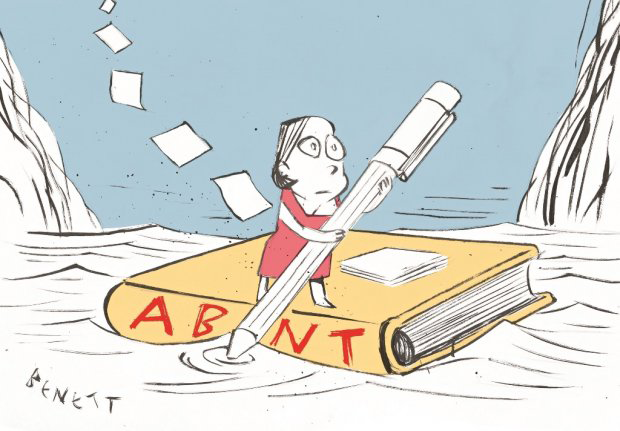
\includegraphics[width=0.8\textwidth]{./04-figuras/navegar_abnt}
    \label{fig:ilustfig}
\end{figure}
\vspace*{-0,9cm}
{\raggedright \fonte{Disponível em: <https://www.gazetadopovo.com.br/abntemfoco>. Acesso em: 24 de jan. de 2015.}}\\

Os títulos devem ser colocados acima das figuras. No texto devem
ser indicados pela pa-lavra Figura acompanhada do número de ordem. E abaixo deve ser indicada sua fonte.

\section{QUADROS}

Denomina-se quadro a apresentação de dados de forma organizada, para cuja compreen-são não seria necessário qualquer elaboração matemático-estatística. A identificação se fará com o nome do elemento Quadro por extenso, seguido do número de ordem em algarismo arábico. Outros elementos do quadro deverão ser descritos de acordo com o padrão usado para
Apresentação tabular.

\begin{quadro}[H]

	\begin{center}
	\caption{Exemplo para quadro.\label{qua:quaexe}}
		\begin{tabular}{|p{7cm}|p{7cm}|}
			\hline
			("Trabalho Conclusão de Curso")\\
			\hline
		\end{tabular}
	\end{center}

\end{quadro}



\section{TABELAS}

Tabelas são conjuntos de dados numéricos, associados a um
fenômeno, dispostos numa determinada ordem da classificação. Expressam as variações qualitativas e quantitativas de um fenômeno. A finalidade básica da tabela é resumir ou sintetizar dados de maneira a fornecer o máximo de informações num mínimo de espaço.

Na apresentação de uma tabela devem ser levados em consideração
os alguns critérios. Toda tabela deve ter significado próprio, dispensando consultas ao texto. A tabela deve ser colo-cada em posição vertical, para facilitar a leitura dos dados. No caso em que isso seja impossível, deve ser colocada em posição horizontal, com o título voltado para a margem esquerda da folha.

Se a tabela ou quadro não couber em uma página, deve ser
continuado na página seguin-te. Neste caso o final não será delimitado por traço horizontal na parte inferior e o cabeçalho será repetido na página seguinte. No texto devem ser indicadas pela palavra Tabela acompanha-da do número de ordem em algarismo arábico.

\begin{table}[H]
    \centering
    \caption[Exemplo tabela]{Exemplo tabela.\label{tab:exetab}}
    \begin{tabular}{cc}
        \hline
            numeros x & numeros y \\
        \hline
            \vspace*{0,15cm} 1 & 15 \vspace*{0,15cm}\\ \hline
            \vspace*{0,15cm} 3 & 4 \vspace*{0,15cm}\\ \hline
            \vspace*{0,15cm} 5 & 6 \vspace*{0,15cm}\\ \hline
            \vspace*{0,15cm} 7 & 8 \vspace*{0,15cm}\\ \hline
			\vspace*{0,15cm} 9 & 11 \vspace*{0,15cm}\\ \hline
            \vspace*{0,15cm} 13 & 15 \vspace*{0,15cm}\\ \hline
        \hline
    \end{tabular}
\end{table}
\vspace*{-0,9cm}
{\raggedright \fonte{Autor desta monografia, 2014.}}

\section{GRÁFICOS}

Depois de sintetizados em tabelas, os dados podem ser
apresentados em gráficos, com a fi-nalidade de proporcionar ao interessado uma visão rápida do comportamento do fenômeno. Serve para representar qualquer tabela de maneira simples, legível e interessante, tornando cla-ros os fatos que poderiam passar despercebidos em dados apenas tabulados.

O elemento de identificação ordenado do gráfico, ou seja, o
número de ordem do mesmo no trabalho. No texto devem ser indicados pela palavra Gráfico, acompanhada do número de ordem em algarismo arábico.



           	% Ilustrações
    %
% Documento: Citações
%

\chapter{CITAÇÕES}

Citação é a menção, no texto, de uma informação colhida de outra fonte. Pode ser direta, indireta e citação de citação. Apresentadas conforme a ABNT NBR 10520

\section{CITAÇÃO DIRETA}

É a transcrição textual dos conceitos de um autor consultado. Um
exemplo: De acordo com as conclusões de Marshall (1980, p. 249) “da mesma forma que não se pode afirmar se é a lâmina inferior ou superior de uma tesoura que corta uma folha de papel, também não se pode discutir se o valor e os preços são governados pela utilidade ou pelo custo de produção”. 

Citação mais longa deve figurar abaixo do texto, em bloco recuado
– de 4 cm da mar-gem esquerda – com letras tamanho 10, sem aspas.

\section{CITAÇÃO INDIRETA}

É a transcrição livre do texto do autor consultado. As citações
indiretas ou parafraseadas dispensam o uso de aspas duplas e do número de páginas.

A produção acadêmica sobre varejo no Brasil fica muito aquem da
importância do seg-mento na economia (ANGELO; SILVA, 1993). É um exemplo de citação indireta.

\section{CITAÇÃO DE CITAÇÃO}

É citação direta ou indireta de um documento ao qual não se teve
acesso aooriginal. De-ve ser citado em nota de rodapé, sendo obrigatória a indicação da Fonte 10 recuo de 4 cm refe-rência de onde foi extraída a informação. Esse tipo de citação só deve ser utilizado nos casos em que realmente o documento original não pode ser recuperado. 

Exemplo: Enguita (apud SILVA, 1991, p. 21) chegou às mesmas
conclusões. As entida-des coletivas podem ser citadas pelas respectivas siglas, desde que na primeira vez em que fo-rem mencionadas apareçam por extenso. Exemplo: ASSOCIAÇÃO BRASILEIRA DO TRA-BALHADOR - ABT (1985)


            	% Citações
    %
% Documento: Tecnicas de referencia
%

\chapter{TÉCNICAS DE REFERÊNCIAS}

É o conjunto padronizado de elementos descritivos, retirados de um documento, que permite a sua identificação individual. Denomina-se ainda de Referências a lista composta de documentos padronizados e utilizados na elaboração de um trabalho acadêmico.

O texto deve estar com o alinhamento justificado, respeitando a formatação indicada pa-ra o tipo de referência. 

\section{MONOGRAFIA}

Monografia Considerada no Todo (livros, folhetos, dissertações,
teses, dicionários, guias). Exemplos: <SOBRENOME, Nome do Autor>. \textbf{Nome
da obra.} Edição.

\section{LIVROS TENDO A ENTIDADE COMO AUTOR}

<NOME DA ENTIDADE>. \textbf{Nome do livro.} Edição.

\section{DOCUMENTOS ELABORADOS POR VÁRIOS AUTORES}

Documentos elaborados por vários autores, com um responsável
intelectual destacado (organizador, coordenador, editor). Exemplo: <SOBRENOME,
Nome do Autor> (Responsabi-lidade atribuída). \textbf{Nome da obra.} Edição.

\section{DOCUMENTOS SEM AUTOR}

<DOCUMENTO e seus subtítulo, caso exista>. Edição. 

\section{ARTIGO OU MATERIA DE REVISTA}

<SOBRENOME, Nome do Autor>. Titulo da matéria. \textbf{Nome da
revista.} Edição.

\section{DOCUMENTO DE EVENTO}

<NOME DO EVENTO, data e local>. Organizador do Evento. Ano,
pagina dos anais onde se encontra a obra. 

\section{EXEMPLOS PARA CITAÇÕES}

Apenas exemplos \cite{7.1.3-1}. Outro \cite{NBR6023:2000}.\cite{NBR10520:1988}. \cite{7.3.2-2}. \cite{7.4.2.1-3}. \cite{7.4.2.1-2}.\cite{7.4.2.3-5}. \cite{7.4.2.1-4}. 
\cite{7.7.1.2-5}. \cite{7.7.1.2-2}. \cite{7.4.2.3-6}. \cite{8.1.1.5}.
            % Tecnica de referencias

    % Elementos pós textuais
    \postextual
    %
% Documento: Referências Bibliográficas
%

\bibliography{refbase}    % Geração automática das referências por meio do arquivo 'refbase.bib'
       % Referências
    %
% Documento: Apêndices
%

\begin{apendicesenv}

    \chapter{Pesquisa de satisfação do Pybot}
    \label{app:quest}

    \begin{table}[H]
    \setlength\extrarowheight{25pt}
    \begin{tabular}{lccccc}
        Profissão:                    & (  )         & \multicolumn{1}{l}{Desenvolvedor}  & (  )         & \multicolumn{1}{l}{Testador}   &              \\
        Facilidade de Instalação:     & 1 $\bigcirc$ & 2 $\bigcirc$                       & 3 $\bigcirc$ & 4 $\bigcirc$                   & 5 $\bigcirc$ \\
        Facilidade de Uso:            & 1 $\bigcirc$ & 2 $\bigcirc$                       & 3 $\bigcirc$ & 4 $\bigcirc$                   & 5 $\bigcirc$ \\
        Atende necessidades básicas:  & 1 $\bigcirc$ & 2 $\bigcirc$                       & 3 $\bigcirc$ & 4 $\bigcirc$                   & 5 $\bigcirc$ \\
        Atende necessidades avançadas & 1 $\bigcirc$ & 2 $\bigcirc$                       & 3 $\bigcirc$ & 4 $\bigcirc$                   & 5 $\bigcirc$ \\
        Comentarios:                  & \multicolumn{5}{l}{\_\_\_\_\_\_\_\_\_\_\_\_\_\_\_\_\_\_\_\_\_\_\_\_\_\_\_\_\_}
    \end{tabular}
    \end{table}

    \chapter{Diagramas de Cenários}
    \label{app:imgs}

    \begin{figure}[H]
        \vspace*{0,3cm}
        \centering
        \caption{Uso padrão Selenium}
        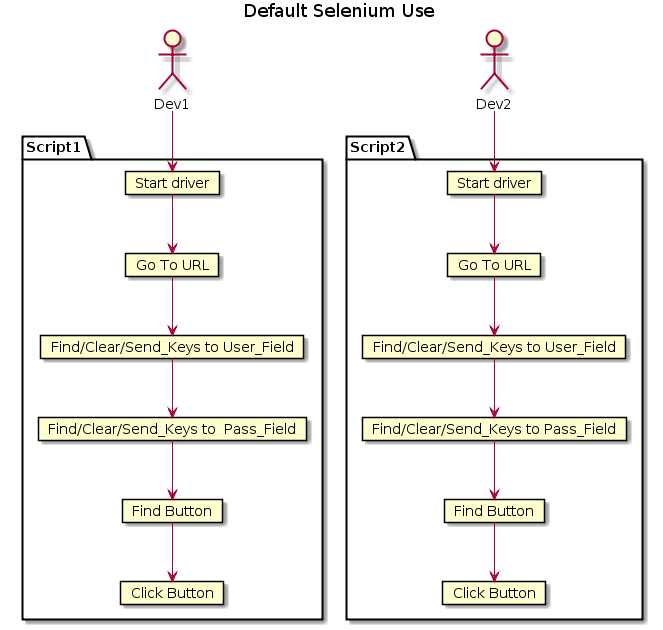
\includegraphics[width=1\textwidth]{./04-figuras/page_object_selenium}
        \label{fig:selenium_default}
    \end{figure}

    \begin{figure}[H]
        \vspace*{0,3cm}
        \centering
        \caption{Uso padrão Selenium com módulo}
        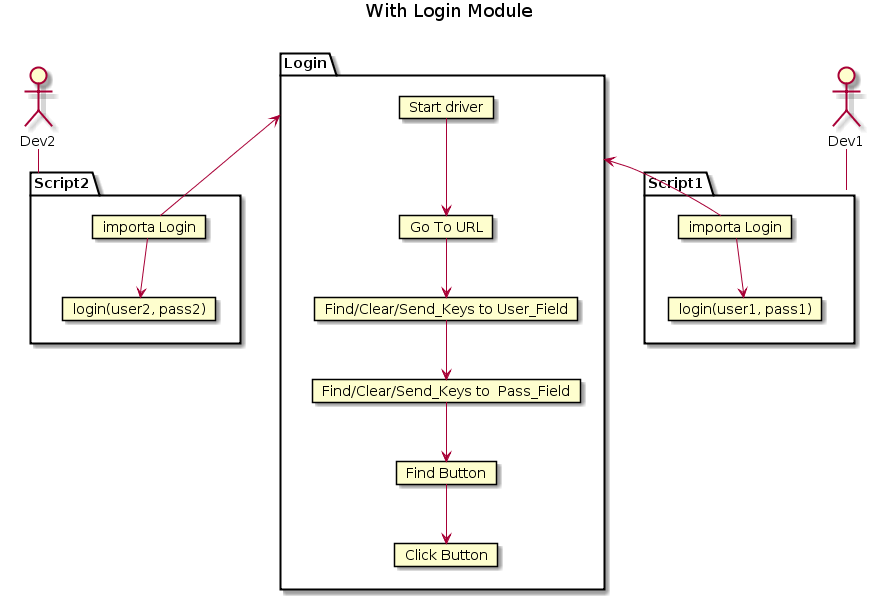
\includegraphics[width=1\textwidth]{./04-figuras/page_object_module}
        \label{fig:selenium_module}
    \end{figure}

    \begin{figure}[H]
        \vspace*{0,3cm}
        \centering
        \caption{Uso padrão Pybot}
        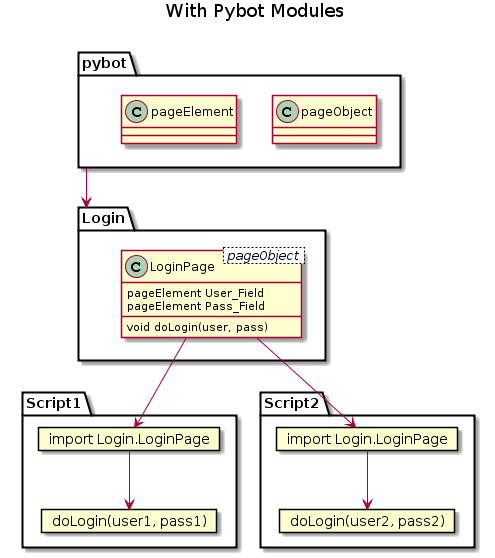
\includegraphics[width=1\textwidth]{./04-figuras/page_object_pybot}
        \label{fig:pybot_module}
    \end{figure}

\end{apendicesenv}         % Apêndices
    %
% Documento: Anexos
%

\begin{anexosenv}

\chapter{Como elaborar}

Anexo é texto ou documento não elaborado pelo autor, que serve de fundamentação, comprovação e ilustração. Elemento opcional. Deve ser precedido da palavra ANEXO, identifi-cado por letras maiúsculas consecutivas, travessão e pelo respectivo título. Utilizam-se letras maiúsculas dobradas, na identificação dos anexos, quando esgotadas as letras do alfabeto.


\end{anexosenv}            % Anexos
    %\printindex                                             % Índice remissivo

\end{document}
